\section{高速化に対する粘度比の影響}
\label{sec:viscosity}
超音波照射による球の高速化度合いは,粘度比$\mu_\text{U}/\mu_\text{ABL}$と音響境界層厚さ$\delta$を球の半径$a$で規格化した値の積で整理できると,先行研究\cite{ref:8}で示唆された.この手法を用いて,第\ref{sec:density},\ref{sec:concentration},\ref{sec:diameter}章に示した各実験結果を整理する.その結果をFig\ref{fig:viscosity_ratio}に示す.

横軸の値が0.2までの範囲において,超音波照射による高速化度合いは,粘度比と音響境界層厚さを球の半径で規格化した値の積に正に相関する.しかし,横軸の値が0.2を越えると,粘度比と音響境界層厚さを球の半径で規格化した値の積に相関が見られない.これより,超音波照射による球の高速化に関して,横軸の値が0.2までの範囲では式(\ref{eq:Udiff})が適用でき,それ以上では,式(\ref{eq:Udiff})が適用できないことが分かった.これは,落下球の半径が小さい場合,擬塑性流体の粘度が大きい場合,落下球と流体の密度差が小さい場合,横軸の値が大きくなる.この要因として,先行研究\cite{ref:8}において弾性による影響が示唆されている.第\ref{sec:elasticity-discussion}章で,それらを議論する.

\begin{figure}[ht]
    \centering
    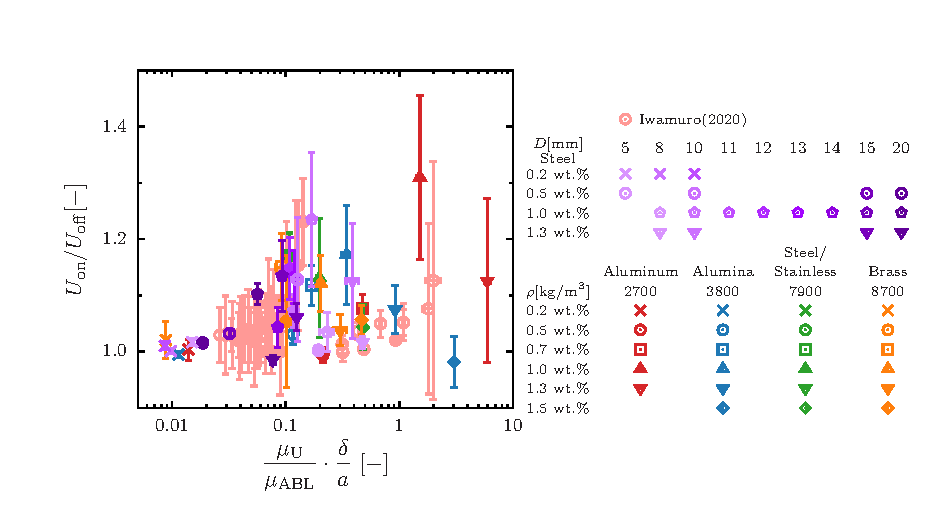
\includegraphics[width=1.0\textwidth]{5-Results/viscosity.eps}
    \caption{Relationship between velocity ratio and the inverse of the viscosity ratio multiplied by the thickness.}
    \label{fig:viscosity_ratio}
\end{figure}
